\section{Results and Discussion}

In this section, we report the findings of our user study comparing the proposed MindMargin interface to the traditional vertical commenting system. Overall, we observed a decrease in polarized views among readers who had seen or read the article previously and an increase in opinion polarization among unfamiliar readers. We also found an increase in readers' positive impressions of comments when using MindMargin. We were able to accept both of our hypotheses.

XXXX "and an increase in opinion polarization among unfamiliar readers" isn't it about the same? no change? XXXX

\subsection{Hypothesis 1}
Our first hypothesis predicted that MindMargin would have an impact on individual opinions, prompting new readers to develop a stance on the issue and encouraging readers with existing views to consider alternate views. The reasoning behind this hypothesis was that MindMargin exposes readers to a greater number of opinions while reading the article. Consequently, readers think more independently, reconsidering their own views in light of others', and develop more thoughtful and nuanced opinions. 

All participants were asked their stance on a Likert scale from Strongly For TFA to Strongly Against TFA. In our analysis, we excluded data from participants who reported to have not read the comments (there was statistically no difference in stance between prototypes Num dropped=XX and Nums for ea. avg stance=XX). We also excluded participants who did not toggle the Likert scale and answer this question (Num==XX). The data of the remaining participants (N=XX) was remapped for their ``Stance Polarization,`` or the deviation of their stance from neutral, as $|50 - stance|$ (range 0-50). 

Participants also reported on their familiarity with the article, which ranged from "read" if they had read or skimmed the article, to "seen" if they had seen the article in the past but did not read or skim it, to "none" if they had never encountered the article prior to this study. We then performed an analysis for both prototypes that included familiarity with the article as a covarying factor and the dependent variable SP, their ``Stance Polarization.`` 

We found that for users whose familiarity of the article was ``none,`` there was no significant difference in the polarization of their stance between MindMargin and the traditional. For participants who were previously exposed to the issue in the article, and whose familiarity with the article was thus ``seen`` or ``read,`` we did in fact observe a difference in stance polarization between the two prototypes (see Figure YYYY). Participants whose familiarity of the article was ``seen`` had a SP value of 7 with MindMargin and 17 with the traditional system. Participants whose familiarity of the article was ``read`` had a SP value of 17 with MindMargin and 27 with the traditional system. The lower SP values among MindMargin users reveal that participants with MindMargin who had prior exposure to the article reported less polarized views to reading the article for a second read or glance. 

However, there are limitations to our observations, as the p-values are XX and XX suggesting that our trends are not yet statistically significant. This could likely result from using a between-subjects methodology. To address this in subsequent research, we plan to significantly increase the participant pool and to employ a within-subjects methodology, in which we query participants for their individual stance prior to their reading of the article and observe the deltas in SP values afterward. 

\subsection{Hypothesis 2}
Our second hypothesis predicted an overall increase in positive impressions on comments when using the MindMargin interface. We asked participants who read the comments to input two adjectives in free-text describing either their reaction to the comments or a description of the comments. We then asked four independent volunteers, blind to the experiment, to classify these adjectives using a four-bin classifier (``Positive,`` ``Negative,`` ``Neutral,`` and ``Invalid``). They were told to classify the adjectives provided that they were in answer to the question, posed on the survey: ``What did you think of the comments (from article X)?`` 

We removed adjectives given two or more ``Invalid`` classifications as outliers, which only appeared in the vertical condition. We found that adjectives without uniform encoding observed an uncontradictory mix of classifications: ``Positive`` and ``Neutral`` or ``Neutral`` and ``Negative,`` but never ``Positive`` and ``Negative.`` We were thus confident in using the resulting median encodings for the final classification of the specified adjectives. 

Then, we compared the impressions between MindMargin and the traditional commenting system. We observed a drastic change of impressions when using MindMargin. As seen in figure \ref{fig:trad_pie}, the majority of participants using the traditional commenting system described the comments as negative (68\%). In contrast, when using MindMargin, the majority of participants described the comments as positive (48\%) or neutral (48\%) as seen in figure \ref{fig:mm_pie}. These results have lead us to conclude that while readers were exposed to identical comments, users of MindMargin had a significantly more positive impression of the comments, considering the comments more substantial and ultimately placing greater trust and consideration into others' opinions.

XXXX aren't we getting rid of the pie charts and those stats? And using ordinal regression of the new data instead? XXXX

\marginpar{
\begin{figure}
  \begin{center}
  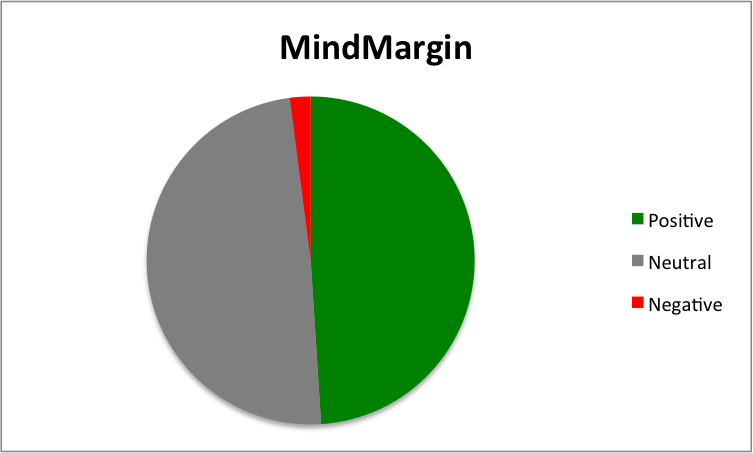
\includegraphics[width=\marginparwidth]{mm_piechart.png}
  \caption{When using MindMargin, the majority of participants described the comments as positive.}
  \label{fig:mm_pie}
  \end{center}
\end{figure}
}

\marginpar{
\begin{figure}
  \begin{center}
  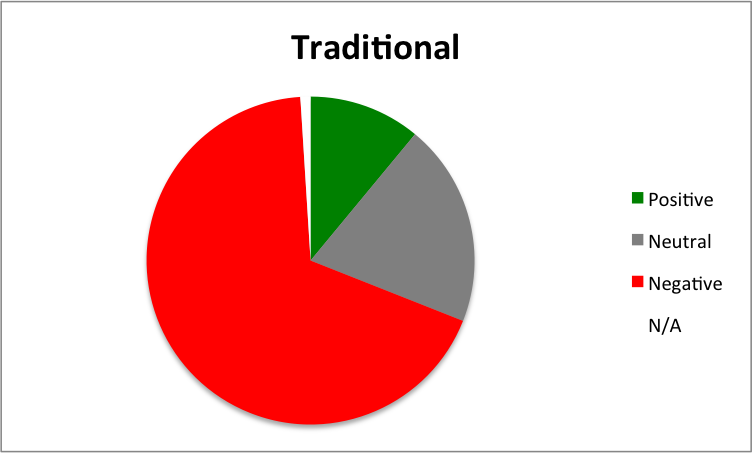
\includegraphics[width=\marginparwidth]{traditional_piechart.png}
  \caption{The majority of participants using the traditional commenting system described the comments as negative.}
  \label{fig:trad_pie}
  \end{center}
\end{figure}
}

In addition to our quantitative results, we would also like to acknowledge qualitative feedback from a MindMargin user that suggests actions he/she took beyond the scope of reading and commenting article:``This article showed me a new perspective on TFA, which after doing research, I have realized I agree with.`` No written feedback suggesting actions outside the scope of the article was received from participants with the traditional commenting system. While there is insufficient evidence to conclude that MindMargin motivated the user's pursuit of further research into the issue, it nevertheless indicates that this reader using MindMargin thought critically and independently about the issue.